\documentclass[]{article}
\usepackage{lmodern}
\usepackage{amssymb,amsmath}
\usepackage{ifxetex,ifluatex}
\usepackage{fixltx2e} % provides \textsubscript
\ifnum 0\ifxetex 1\fi\ifluatex 1\fi=0 % if pdftex
  \usepackage[T1]{fontenc}
  \usepackage[utf8]{inputenc}
\else % if luatex or xelatex
  \ifxetex
    \usepackage{mathspec}
  \else
    \usepackage{fontspec}
  \fi
  \defaultfontfeatures{Ligatures=TeX,Scale=MatchLowercase}
\fi
% use upquote if available, for straight quotes in verbatim environments
\IfFileExists{upquote.sty}{\usepackage{upquote}}{}
% use microtype if available
\IfFileExists{microtype.sty}{%
\usepackage{microtype}
\UseMicrotypeSet[protrusion]{basicmath} % disable protrusion for tt fonts
}{}
\usepackage[margin=1in]{geometry}
\usepackage{hyperref}
\hypersetup{unicode=true,
            pdftitle={MVA Final Project},
            pdfauthor={Javier Ferrando Monsonis; Marcel Porta Valles; Mehmet Fatih ??agil},
            pdfborder={0 0 0},
            breaklinks=true}
\urlstyle{same}  % don't use monospace font for urls
\usepackage{color}
\usepackage{fancyvrb}
\newcommand{\VerbBar}{|}
\newcommand{\VERB}{\Verb[commandchars=\\\{\}]}
\DefineVerbatimEnvironment{Highlighting}{Verbatim}{commandchars=\\\{\}}
% Add ',fontsize=\small' for more characters per line
\usepackage{framed}
\definecolor{shadecolor}{RGB}{248,248,248}
\newenvironment{Shaded}{\begin{snugshade}}{\end{snugshade}}
\newcommand{\KeywordTok}[1]{\textcolor[rgb]{0.13,0.29,0.53}{\textbf{#1}}}
\newcommand{\DataTypeTok}[1]{\textcolor[rgb]{0.13,0.29,0.53}{#1}}
\newcommand{\DecValTok}[1]{\textcolor[rgb]{0.00,0.00,0.81}{#1}}
\newcommand{\BaseNTok}[1]{\textcolor[rgb]{0.00,0.00,0.81}{#1}}
\newcommand{\FloatTok}[1]{\textcolor[rgb]{0.00,0.00,0.81}{#1}}
\newcommand{\ConstantTok}[1]{\textcolor[rgb]{0.00,0.00,0.00}{#1}}
\newcommand{\CharTok}[1]{\textcolor[rgb]{0.31,0.60,0.02}{#1}}
\newcommand{\SpecialCharTok}[1]{\textcolor[rgb]{0.00,0.00,0.00}{#1}}
\newcommand{\StringTok}[1]{\textcolor[rgb]{0.31,0.60,0.02}{#1}}
\newcommand{\VerbatimStringTok}[1]{\textcolor[rgb]{0.31,0.60,0.02}{#1}}
\newcommand{\SpecialStringTok}[1]{\textcolor[rgb]{0.31,0.60,0.02}{#1}}
\newcommand{\ImportTok}[1]{#1}
\newcommand{\CommentTok}[1]{\textcolor[rgb]{0.56,0.35,0.01}{\textit{#1}}}
\newcommand{\DocumentationTok}[1]{\textcolor[rgb]{0.56,0.35,0.01}{\textbf{\textit{#1}}}}
\newcommand{\AnnotationTok}[1]{\textcolor[rgb]{0.56,0.35,0.01}{\textbf{\textit{#1}}}}
\newcommand{\CommentVarTok}[1]{\textcolor[rgb]{0.56,0.35,0.01}{\textbf{\textit{#1}}}}
\newcommand{\OtherTok}[1]{\textcolor[rgb]{0.56,0.35,0.01}{#1}}
\newcommand{\FunctionTok}[1]{\textcolor[rgb]{0.00,0.00,0.00}{#1}}
\newcommand{\VariableTok}[1]{\textcolor[rgb]{0.00,0.00,0.00}{#1}}
\newcommand{\ControlFlowTok}[1]{\textcolor[rgb]{0.13,0.29,0.53}{\textbf{#1}}}
\newcommand{\OperatorTok}[1]{\textcolor[rgb]{0.81,0.36,0.00}{\textbf{#1}}}
\newcommand{\BuiltInTok}[1]{#1}
\newcommand{\ExtensionTok}[1]{#1}
\newcommand{\PreprocessorTok}[1]{\textcolor[rgb]{0.56,0.35,0.01}{\textit{#1}}}
\newcommand{\AttributeTok}[1]{\textcolor[rgb]{0.77,0.63,0.00}{#1}}
\newcommand{\RegionMarkerTok}[1]{#1}
\newcommand{\InformationTok}[1]{\textcolor[rgb]{0.56,0.35,0.01}{\textbf{\textit{#1}}}}
\newcommand{\WarningTok}[1]{\textcolor[rgb]{0.56,0.35,0.01}{\textbf{\textit{#1}}}}
\newcommand{\AlertTok}[1]{\textcolor[rgb]{0.94,0.16,0.16}{#1}}
\newcommand{\ErrorTok}[1]{\textcolor[rgb]{0.64,0.00,0.00}{\textbf{#1}}}
\newcommand{\NormalTok}[1]{#1}
\usepackage{longtable,booktabs}
\usepackage{graphicx,grffile}
\makeatletter
\def\maxwidth{\ifdim\Gin@nat@width>\linewidth\linewidth\else\Gin@nat@width\fi}
\def\maxheight{\ifdim\Gin@nat@height>\textheight\textheight\else\Gin@nat@height\fi}
\makeatother
% Scale images if necessary, so that they will not overflow the page
% margins by default, and it is still possible to overwrite the defaults
% using explicit options in \includegraphics[width, height, ...]{}
\setkeys{Gin}{width=\maxwidth,height=\maxheight,keepaspectratio}
\IfFileExists{parskip.sty}{%
\usepackage{parskip}
}{% else
\setlength{\parindent}{0pt}
\setlength{\parskip}{6pt plus 2pt minus 1pt}
}
\setlength{\emergencystretch}{3em}  % prevent overfull lines
\providecommand{\tightlist}{%
  \setlength{\itemsep}{0pt}\setlength{\parskip}{0pt}}
\setcounter{secnumdepth}{0}
% Redefines (sub)paragraphs to behave more like sections
\ifx\paragraph\undefined\else
\let\oldparagraph\paragraph
\renewcommand{\paragraph}[1]{\oldparagraph{#1}\mbox{}}
\fi
\ifx\subparagraph\undefined\else
\let\oldsubparagraph\subparagraph
\renewcommand{\subparagraph}[1]{\oldsubparagraph{#1}\mbox{}}
\fi

%%% Use protect on footnotes to avoid problems with footnotes in titles
\let\rmarkdownfootnote\footnote%
\def\footnote{\protect\rmarkdownfootnote}

%%% Change title format to be more compact
\usepackage{titling}

% Create subtitle command for use in maketitle
\newcommand{\subtitle}[1]{
  \posttitle{
    \begin{center}\large#1\end{center}
    }
}

\setlength{\droptitle}{-2em}

  \title{MVA Final Project}
    \pretitle{\vspace{\droptitle}\centering\huge}
  \posttitle{\par}
    \author{Javier Ferrando Monsonis \\ Marcel Porta Valles \\ Mehmet Fatih ??agil}
    \preauthor{\centering\large\emph}
  \postauthor{\par}
      \predate{\centering\large\emph}
  \postdate{\par}
    \date{February 20, 2018}


\begin{document}
\maketitle

\subsection{Libraries}\label{libraries}

\begin{Shaded}
\begin{Highlighting}[]
\KeywordTok{library}\NormalTok{(chemometrics)}
\KeywordTok{library}\NormalTok{(DMwR)}
\KeywordTok{library}\NormalTok{(mice)}
\KeywordTok{library}\NormalTok{(missForest)}
\KeywordTok{library}\NormalTok{(ggplot2)}
\KeywordTok{library}\NormalTok{(graphics)}
\KeywordTok{library}\NormalTok{(gridExtra)}
\KeywordTok{library}\NormalTok{(Hmisc)}
\KeywordTok{library}\NormalTok{(knitr)}
\KeywordTok{library}\NormalTok{(FactoMineR)}
\KeywordTok{library}\NormalTok{(DataExplorer)}
\end{Highlighting}
\end{Shaded}

\begin{verbatim}
## Warning: package 'DataExplorer' was built under R version 3.5.2
\end{verbatim}

\begin{Shaded}
\begin{Highlighting}[]
\KeywordTok{library}\NormalTok{(factoextra)}
\KeywordTok{library}\NormalTok{(expm)}
\KeywordTok{library}\NormalTok{(fpc)}
\KeywordTok{library}\NormalTok{(cluster)}

\KeywordTok{theme_set}\NormalTok{(}\KeywordTok{theme_bw}\NormalTok{())}
\KeywordTok{setwd}\NormalTok{(}\StringTok{"/Users/JaviFerrando/Desktop/MVA-Project"}\NormalTok{)}
\end{Highlighting}
\end{Shaded}

\begin{Shaded}
\begin{Highlighting}[]
\NormalTok{heart_disease =}\StringTok{ }\KeywordTok{read.csv}\NormalTok{(}\StringTok{"data/heart.csv"}\NormalTok{)}
\NormalTok{columns <-}\StringTok{ }\KeywordTok{colnames}\NormalTok{(heart_disease)}
\NormalTok{columns[}\DecValTok{1}\NormalTok{] <-}\StringTok{ "age"}
\KeywordTok{colnames}\NormalTok{(heart_disease) <-}\StringTok{ }\NormalTok{columns}

\CommentTok{# Find missing variables}
\KeywordTok{which}\NormalTok{(}\KeywordTok{is.na}\NormalTok{(heart_disease))}
\end{Highlighting}
\end{Shaded}

\begin{verbatim}
## integer(0)
\end{verbatim}

\begin{Shaded}
\begin{Highlighting}[]
\KeywordTok{kable}\NormalTok{(}\KeywordTok{head}\NormalTok{(heart_disease))}
\end{Highlighting}
\end{Shaded}

\begin{longtable}[]{@{}rrrrrrrrrrrrrr@{}}
\toprule
age & sex & cp & trestbps & chol & fbs & restecg & thalach & exang &
oldpeak & slope & ca & thal & target\tabularnewline
\midrule
\endhead
63 & 1 & 3 & 145 & 233 & 1 & 0 & 150 & 0 & 2.3 & 0 & 0 & 1 &
1\tabularnewline
37 & 1 & 2 & 130 & 250 & 0 & 1 & 187 & 0 & 3.5 & 0 & 0 & 2 &
1\tabularnewline
41 & 0 & 1 & 130 & 204 & 0 & 0 & 172 & 0 & 1.4 & 2 & 0 & 2 &
1\tabularnewline
56 & 1 & 1 & 120 & 236 & 0 & 1 & 178 & 0 & 0.8 & 2 & 0 & 2 &
1\tabularnewline
57 & 0 & 0 & 120 & 354 & 0 & 1 & 163 & 1 & 0.6 & 2 & 0 & 2 &
1\tabularnewline
57 & 1 & 0 & 140 & 192 & 0 & 1 & 148 & 0 & 0.4 & 1 & 0 & 1 &
1\tabularnewline
\bottomrule
\end{longtable}

\begin{Shaded}
\begin{Highlighting}[]
\KeywordTok{describe}\NormalTok{(heart_disease)}
\end{Highlighting}
\end{Shaded}

\begin{verbatim}
## heart_disease 
## 
##  14  Variables      303  Observations
## ---------------------------------------------------------------------------
## age 
##        n  missing distinct     Info     Mean      Gmd      .05      .10 
##      303        0       41    0.999    54.37    10.36     39.1     42.0 
##      .25      .50      .75      .90      .95 
##     47.5     55.0     61.0     66.0     68.0 
## 
## lowest : 29 34 35 37 38, highest: 70 71 74 76 77
## ---------------------------------------------------------------------------
## sex 
##        n  missing distinct     Info      Sum     Mean      Gmd 
##      303        0        2    0.649      207   0.6832   0.4343 
## 
## ---------------------------------------------------------------------------
## cp 
##        n  missing distinct     Info     Mean      Gmd 
##      303        0        4    0.866    0.967    1.105 
##                                   
## Value          0     1     2     3
## Frequency    143    50    87    23
## Proportion 0.472 0.165 0.287 0.076
## ---------------------------------------------------------------------------
## trestbps 
##        n  missing distinct     Info     Mean      Gmd      .05      .10 
##      303        0       49    0.995    131.6    19.32      108      110 
##      .25      .50      .75      .90      .95 
##      120      130      140      152      160 
## 
## lowest :  94 100 101 102 104, highest: 174 178 180 192 200
## ---------------------------------------------------------------------------
## chol 
##        n  missing distinct     Info     Mean      Gmd      .05      .10 
##      303        0      152        1    246.3    55.95    175.0    188.0 
##      .25      .50      .75      .90      .95 
##    211.0    240.0    274.5    308.8    326.9 
## 
## lowest : 126 131 141 149 157, highest: 394 407 409 417 564
## ---------------------------------------------------------------------------
## fbs 
##        n  missing distinct     Info      Sum     Mean      Gmd 
##      303        0        2    0.379       45   0.1485   0.2538 
## 
## ---------------------------------------------------------------------------
## restecg 
##        n  missing distinct     Info     Mean      Gmd 
##      303        0        3     0.76   0.5281   0.5274 
##                             
## Value          0     1     2
## Frequency    147   152     4
## Proportion 0.485 0.502 0.013
## ---------------------------------------------------------------------------
## thalach 
##        n  missing distinct     Info     Mean      Gmd      .05      .10 
##      303        0       91        1    149.6    25.77    108.1    116.0 
##      .25      .50      .75      .90      .95 
##    133.5    153.0    166.0    176.6    181.9 
## 
## lowest :  71  88  90  95  96, highest: 190 192 194 195 202
## ---------------------------------------------------------------------------
## exang 
##        n  missing distinct     Info      Sum     Mean      Gmd 
##      303        0        2     0.66       99   0.3267   0.4414 
## 
## ---------------------------------------------------------------------------
## oldpeak 
##        n  missing distinct     Info     Mean      Gmd      .05      .10 
##      303        0       40    0.964     1.04    1.225      0.0      0.0 
##      .25      .50      .75      .90      .95 
##      0.0      0.8      1.6      2.8      3.4 
## 
## lowest : 0.0 0.1 0.2 0.3 0.4, highest: 4.0 4.2 4.4 5.6 6.2
## ---------------------------------------------------------------------------
## slope 
##        n  missing distinct     Info     Mean      Gmd 
##      303        0        3    0.798    1.399   0.6291 
##                             
## Value          0     1     2
## Frequency     21   140   142
## Proportion 0.069 0.462 0.469
## ---------------------------------------------------------------------------
## ca 
##        n  missing distinct     Info     Mean      Gmd 
##      303        0        5    0.795   0.7294    1.005 
##                                         
## Value          0     1     2     3     4
## Frequency    175    65    38    20     5
## Proportion 0.578 0.215 0.125 0.066 0.017
## ---------------------------------------------------------------------------
## thal 
##        n  missing distinct     Info     Mean      Gmd 
##      303        0        4    0.778    2.314   0.6125 
##                                   
## Value          0     1     2     3
## Frequency      2    18   166   117
## Proportion 0.007 0.059 0.548 0.386
## ---------------------------------------------------------------------------
## target 
##        n  missing distinct     Info      Sum     Mean      Gmd 
##      303        0        2    0.744      165   0.5446   0.4977 
## 
## ---------------------------------------------------------------------------
\end{verbatim}

\begin{Shaded}
\begin{Highlighting}[]
\NormalTok{classVar <-}\StringTok{ }\KeywordTok{lapply}\NormalTok{(heart_disease,class)   }\CommentTok{# class of each variable}
\NormalTok{factor_heart <-}\StringTok{ }\NormalTok{heart_disease}
\NormalTok{factor_heart}\OperatorTok{$}\NormalTok{target <-}\StringTok{ }\KeywordTok{as.factor}\NormalTok{(heart_disease}\OperatorTok{$}\NormalTok{target)}
\NormalTok{factor_heart}\OperatorTok{$}\NormalTok{sex <-}\StringTok{ }\KeywordTok{as.factor}\NormalTok{(heart_disease}\OperatorTok{$}\NormalTok{sex)}
\NormalTok{factor_heart}\OperatorTok{$}\NormalTok{fbs <-}\StringTok{ }\KeywordTok{as.factor}\NormalTok{(heart_disease}\OperatorTok{$}\NormalTok{fbs)}
\NormalTok{factor_heart}\OperatorTok{$}\NormalTok{exang <-}\StringTok{ }\KeywordTok{as.factor}\NormalTok{(heart_disease}\OperatorTok{$}\NormalTok{exang)}
\NormalTok{factor_heart}\OperatorTok{$}\NormalTok{restecg <-}\StringTok{ }\KeywordTok{as.factor}\NormalTok{(heart_disease}\OperatorTok{$}\NormalTok{restecg)}
\NormalTok{factor_heart}\OperatorTok{$}\NormalTok{thal <-}\StringTok{ }\KeywordTok{as.factor}\NormalTok{(heart_disease}\OperatorTok{$}\NormalTok{thal)}
\NormalTok{factor_heart}\OperatorTok{$}\NormalTok{slope <-}\StringTok{ }\KeywordTok{as.factor}\NormalTok{(heart_disease}\OperatorTok{$}\NormalTok{slope)}
\NormalTok{factor_heart}\OperatorTok{$}\NormalTok{cp <-}\StringTok{ }\KeywordTok{as.factor}\NormalTok{(heart_disease}\OperatorTok{$}\NormalTok{cp)}
\NormalTok{factor_heart}\OperatorTok{$}\NormalTok{ca <-}\StringTok{ }\KeywordTok{as.factor}\NormalTok{(heart_disease}\OperatorTok{$}\NormalTok{ca)}
\end{Highlighting}
\end{Shaded}

\begin{Shaded}
\begin{Highlighting}[]
\CommentTok{#Outlier detection}
\NormalTok{############################}
\CommentTok{#Moutlier(heart_disease[,-14], quantile = 0.975, plot = TRUE, tol=1e-36) #Doesn't work}


\CommentTok{#Local Outlier Factor}
\NormalTok{outlier.scores <-}\StringTok{ }\KeywordTok{lofactor}\NormalTok{(heart_disease[,}\OperatorTok{-}\DecValTok{14}\NormalTok{], }\DataTypeTok{k=}\DecValTok{5}\NormalTok{)}
\KeywordTok{plot}\NormalTok{(}\KeywordTok{density}\NormalTok{(outlier.scores),}\DataTypeTok{main=}\StringTok{'Distribution of individuals local outlier factor scores'}\NormalTok{)}
\end{Highlighting}
\end{Shaded}

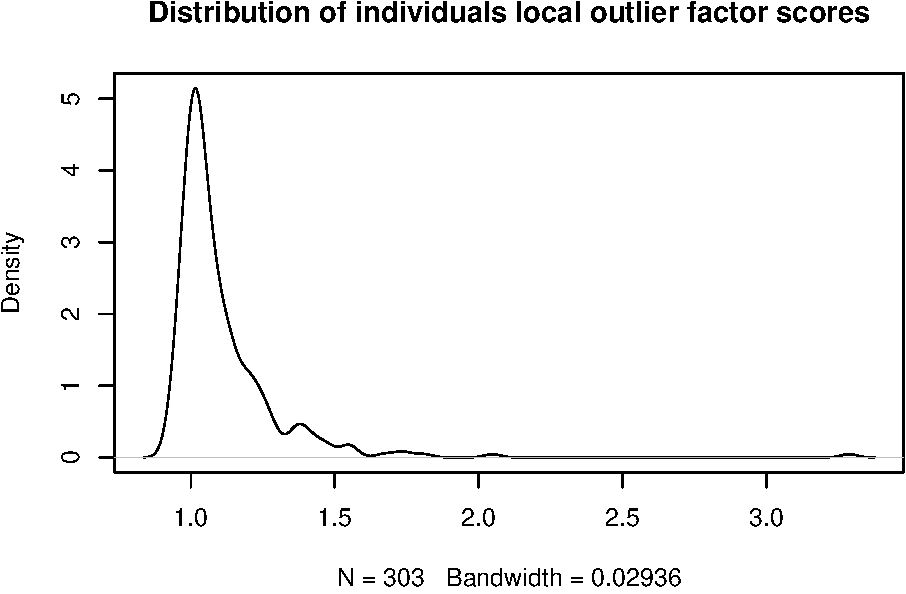
\includegraphics{project_report_files/figure-latex/unnamed-chunk-4-1.pdf}

\begin{Shaded}
\begin{Highlighting}[]
\CommentTok{#Exploratory Data Analysis}
\CommentTok{#Density of heart presence/absence disease by age}
\NormalTok{g1 <-}\StringTok{ }\KeywordTok{ggplot}\NormalTok{(}\DataTypeTok{data=}\NormalTok{heart_disease, }\KeywordTok{aes}\NormalTok{(}\DataTypeTok{x=}\NormalTok{age, }\DataTypeTok{fill=}\KeywordTok{as.factor}\NormalTok{(target)))}\OperatorTok{+}
\StringTok{  }\KeywordTok{geom_density}\NormalTok{(}\DataTypeTok{alpha=}\NormalTok{.}\DecValTok{5}\NormalTok{)}\OperatorTok{+}
\StringTok{  }\KeywordTok{ggtitle}\NormalTok{(}\StringTok{"Age"}\NormalTok{) }\OperatorTok{+}
\StringTok{  }\KeywordTok{scale_fill_manual}\NormalTok{(}\DataTypeTok{values =} \KeywordTok{c}\NormalTok{(}\StringTok{'skyblue4'}\NormalTok{, }\StringTok{'skyblue2'}\NormalTok{),}\DataTypeTok{name =} \StringTok{"Disease"}\NormalTok{, }\DataTypeTok{labels =} \KeywordTok{c}\NormalTok{(}\StringTok{"Yes"}\NormalTok{, }\StringTok{"No"}\NormalTok{))}

\CommentTok{#Density of heart presence/absence disease by Max heart rate}
\NormalTok{g2 <-}\StringTok{ }\KeywordTok{ggplot}\NormalTok{(}\DataTypeTok{data=}\NormalTok{heart_disease, }\KeywordTok{aes}\NormalTok{(}\DataTypeTok{x=}\NormalTok{thalach, }\DataTypeTok{fill=}\KeywordTok{as.factor}\NormalTok{(target)))}\OperatorTok{+}
\StringTok{  }\KeywordTok{geom_density}\NormalTok{(}\DataTypeTok{alpha=}\NormalTok{.}\DecValTok{5}\NormalTok{)}\OperatorTok{+}
\StringTok{  }\KeywordTok{ggtitle}\NormalTok{(}\StringTok{"Max Hear Rate"}\NormalTok{) }\OperatorTok{+}
\StringTok{  }\KeywordTok{scale_fill_manual}\NormalTok{(}\DataTypeTok{values =} \KeywordTok{c}\NormalTok{(}\StringTok{'skyblue4'}\NormalTok{, }\StringTok{'skyblue2'}\NormalTok{),}\DataTypeTok{name =} \StringTok{"Disease"}\NormalTok{, }\DataTypeTok{labels =} \KeywordTok{c}\NormalTok{(}\StringTok{"Yes"}\NormalTok{, }\StringTok{"No"}\NormalTok{))}

\CommentTok{#Density of heart presence/absence disease by sex}
\NormalTok{g3 <-}\StringTok{ }\KeywordTok{ggplot}\NormalTok{(}\DataTypeTok{data=}\NormalTok{heart_disease, }\KeywordTok{aes}\NormalTok{(}\DataTypeTok{x=}\NormalTok{sex, }\DataTypeTok{fill=}\KeywordTok{as.factor}\NormalTok{(target)))}\OperatorTok{+}
\StringTok{      }\KeywordTok{geom_bar}\NormalTok{(}\DataTypeTok{alpha=}\NormalTok{.}\DecValTok{5}\NormalTok{, }\DataTypeTok{color=}\StringTok{"black"}\NormalTok{)}\OperatorTok{+}
\StringTok{      }\KeywordTok{ggtitle}\NormalTok{(}\StringTok{"Sex"}\NormalTok{) }\OperatorTok{+}
\StringTok{      }\KeywordTok{scale_fill_manual}\NormalTok{(}\DataTypeTok{values =} \KeywordTok{c}\NormalTok{(}\StringTok{'skyblue4'}\NormalTok{, }\StringTok{'skyblue2'}\NormalTok{),}\DataTypeTok{name =} \StringTok{"Disease"}\NormalTok{, }\DataTypeTok{labels =} \KeywordTok{c}\NormalTok{(}\StringTok{"Yes"}\NormalTok{, }\StringTok{"No"}\NormalTok{))}

\CommentTok{#Density of heart presence/absence disease by chest type}
\NormalTok{g4 <-}\StringTok{ }\KeywordTok{ggplot}\NormalTok{(}\DataTypeTok{data=}\NormalTok{heart_disease, }\KeywordTok{aes}\NormalTok{(}\DataTypeTok{x=}\NormalTok{cp, }\DataTypeTok{fill=}\KeywordTok{as.factor}\NormalTok{(target)))}\OperatorTok{+}
\StringTok{  }\KeywordTok{geom_bar}\NormalTok{(}\DataTypeTok{alpha=}\NormalTok{.}\DecValTok{5}\NormalTok{, }\DataTypeTok{color=}\StringTok{"black"}\NormalTok{)}\OperatorTok{+}
\StringTok{  }\KeywordTok{ggtitle}\NormalTok{(}\StringTok{"Chest Pain type"}\NormalTok{) }\OperatorTok{+}
\StringTok{  }\KeywordTok{scale_fill_manual}\NormalTok{(}\DataTypeTok{values =} \KeywordTok{c}\NormalTok{(}\StringTok{'skyblue4'}\NormalTok{, }\StringTok{'skyblue2'}\NormalTok{),}\DataTypeTok{name =} \StringTok{"Disease"}\NormalTok{, }\DataTypeTok{labels =} \KeywordTok{c}\NormalTok{(}\StringTok{"Yes"}\NormalTok{, }\StringTok{"No"}\NormalTok{))}

\KeywordTok{grid.arrange}\NormalTok{(g1, g2, g3, g4, }\DataTypeTok{ncol =} \DecValTok{2}\NormalTok{)}
\end{Highlighting}
\end{Shaded}

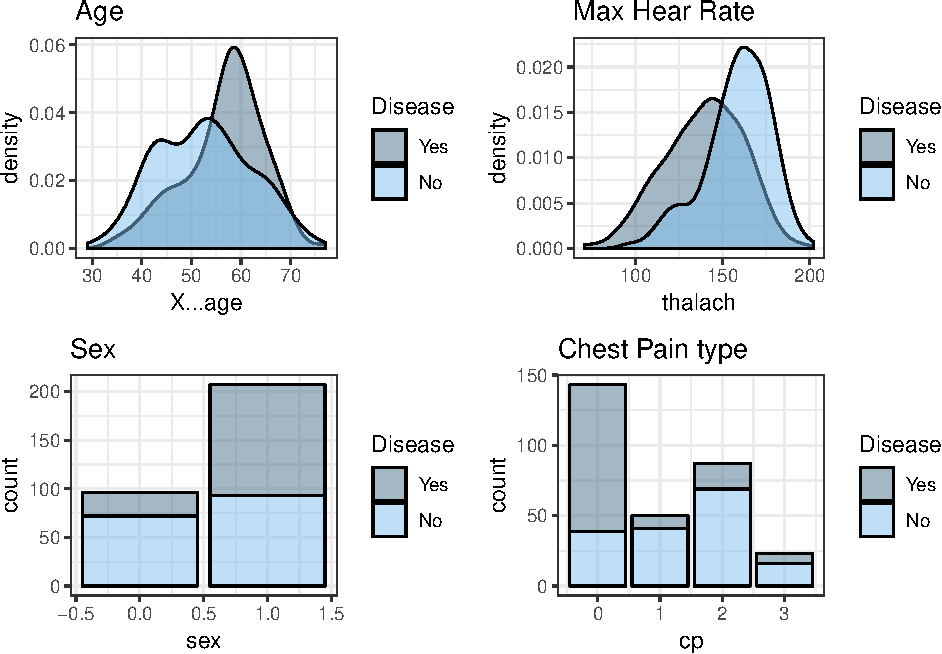
\includegraphics{project_report_files/figure-latex/unnamed-chunk-5-1.pdf}

\begin{Shaded}
\begin{Highlighting}[]
\KeywordTok{plot_correlation}\NormalTok{(heart_disease)}
\end{Highlighting}
\end{Shaded}

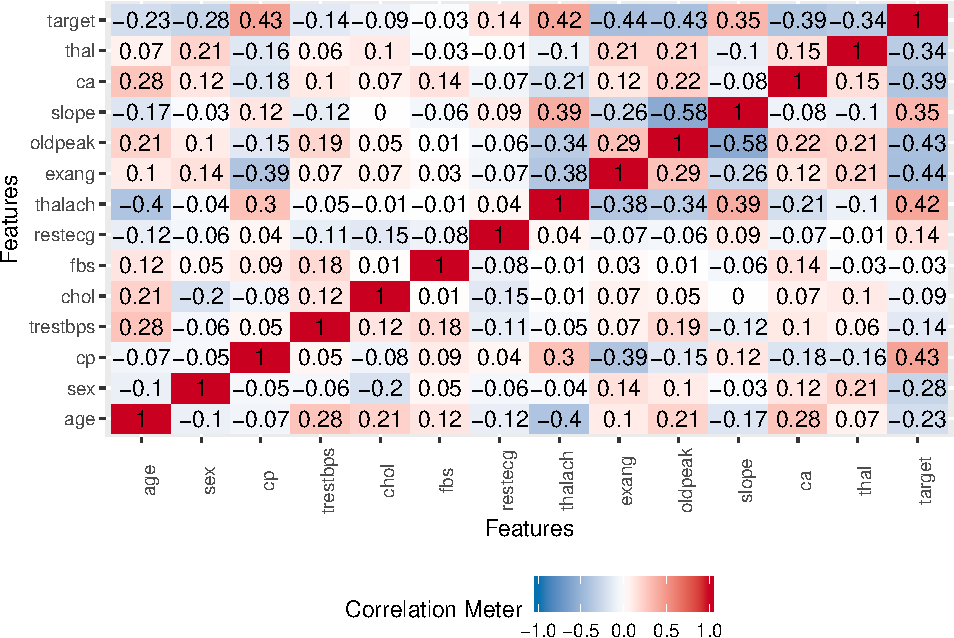
\includegraphics{project_report_files/figure-latex/unnamed-chunk-6-1.pdf}

\begin{Shaded}
\begin{Highlighting}[]
\CommentTok{#PCA with categoriacal values}
\NormalTok{pca_facto <-}\StringTok{ }\NormalTok{factor_heart[, }\KeywordTok{sapply}\NormalTok{(factor_heart, class) }\OperatorTok{!=}\StringTok{ "factor"}\NormalTok{]}
\CommentTok{#Some categorical values can be added as supplementary}
\CommentTok{#pca_facto$sex <- factor_heart$sex}
\CommentTok{#pca_facto$ca <- factor_heart$ca}
\NormalTok{pca_facto}\OperatorTok{$}\NormalTok{disease <-}\StringTok{ }\NormalTok{heart_disease}\OperatorTok{$}\NormalTok{target}
\NormalTok{pca_facto}\OperatorTok{$}\NormalTok{disease[pca_facto}\OperatorTok{$}\NormalTok{disease}\OperatorTok{==}\DecValTok{0}\NormalTok{] <-}\StringTok{ "Yes"}
\NormalTok{pca_facto}\OperatorTok{$}\NormalTok{disease[pca_facto}\OperatorTok{$}\NormalTok{disease}\OperatorTok{==}\DecValTok{1}\NormalTok{] <-}\StringTok{ "No"}

\NormalTok{pca_facto_heart <-}\StringTok{ }\KeywordTok{PCA}\NormalTok{(pca_facto, }\DataTypeTok{quali.sup =} \DecValTok{6}\NormalTok{, }\DataTypeTok{scale.unit =} \OtherTok{TRUE}\NormalTok{,  }\DataTypeTok{graph =} \OtherTok{TRUE}\NormalTok{)}
\end{Highlighting}
\end{Shaded}

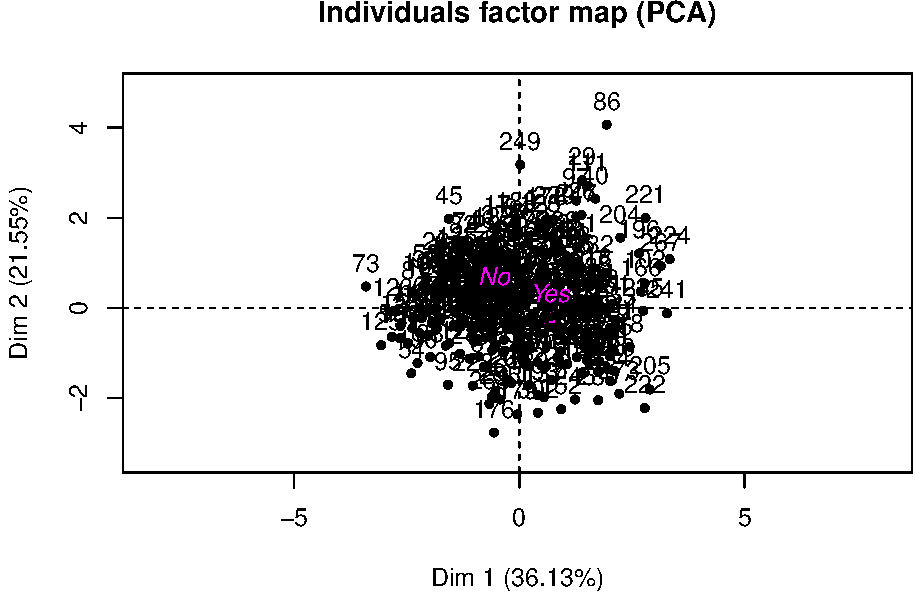
\includegraphics{project_report_files/figure-latex/unnamed-chunk-7-1.pdf}
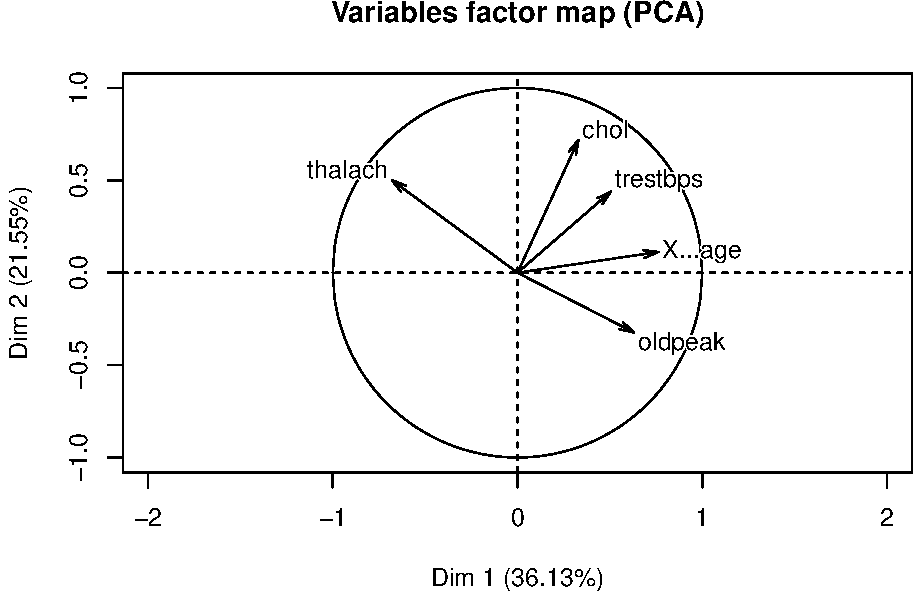
\includegraphics{project_report_files/figure-latex/unnamed-chunk-7-2.pdf}

\begin{Shaded}
\begin{Highlighting}[]
\CommentTok{#Screeplots}
\KeywordTok{fviz_screeplot}\NormalTok{(pca_facto_heart, }\DataTypeTok{addlabels =} \OtherTok{FALSE}\NormalTok{)}
\end{Highlighting}
\end{Shaded}

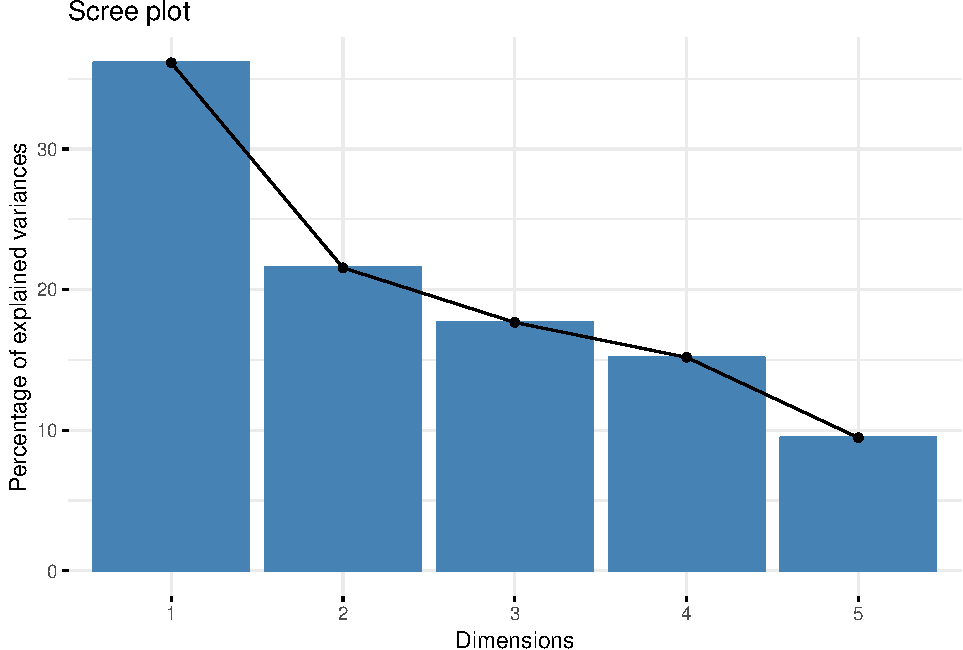
\includegraphics{project_report_files/figure-latex/unnamed-chunk-8-1.pdf}

\begin{Shaded}
\begin{Highlighting}[]
\NormalTok{eigen_values <-}\StringTok{ }\NormalTok{pca_facto_heart}\OperatorTok{$}\NormalTok{eig[,}\DecValTok{1}\NormalTok{]}
\KeywordTok{plot}\NormalTok{(eigen_values, }\DataTypeTok{type=}\StringTok{"o"}\NormalTok{, }\DataTypeTok{main=}\StringTok{"Screeplot"}\NormalTok{, }
     \DataTypeTok{xlab=}\StringTok{'Dimension'}\NormalTok{, }\DataTypeTok{ylab=}\StringTok{'Eigenvalue'}\NormalTok{, }\DataTypeTok{col=}\StringTok{'blue'}\NormalTok{)}
\KeywordTok{abline}\NormalTok{(}\DataTypeTok{h=}\DecValTok{1}\NormalTok{,}\DataTypeTok{col=}\StringTok{"red"}\NormalTok{)}
\end{Highlighting}
\end{Shaded}

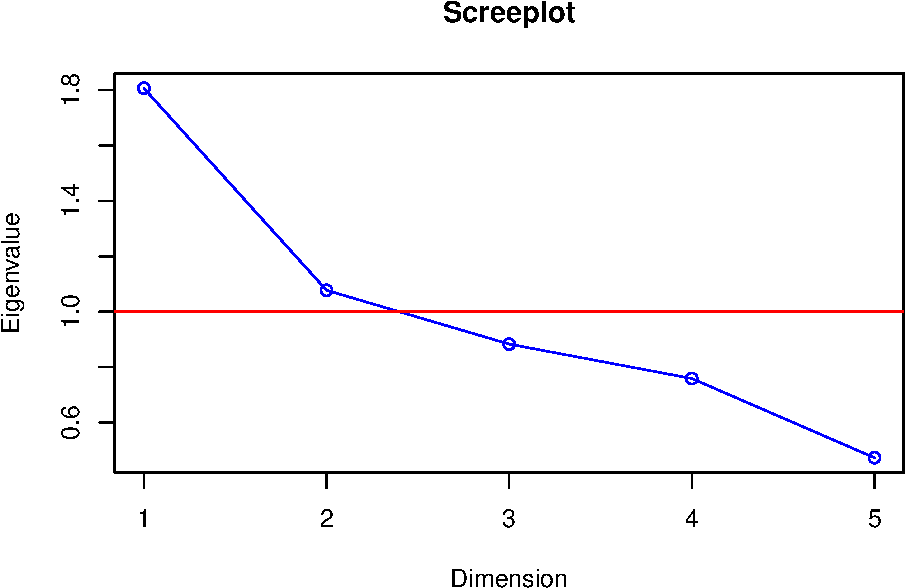
\includegraphics{project_report_files/figure-latex/unnamed-chunk-8-2.pdf}

\begin{Shaded}
\begin{Highlighting}[]
\CommentTok{#Represented in Rp}
\CommentTok{#quali.sup -> Every modality is the centroide of the respective individuals having chosen that modality}
\KeywordTok{fviz_pca_ind}\NormalTok{(pca_facto_heart, }\DataTypeTok{habillage =} \DecValTok{6}\NormalTok{, }\DataTypeTok{geom =} \StringTok{"point"}\NormalTok{, }\DataTypeTok{label=}\StringTok{"quali"}\NormalTok{,}\DataTypeTok{addEllipses =}\OtherTok{TRUE}\NormalTok{, }\DataTypeTok{ellipse.level =} \FloatTok{0.68}\NormalTok{)}\CommentTok{#co l.ind='cos2'}
\end{Highlighting}
\end{Shaded}

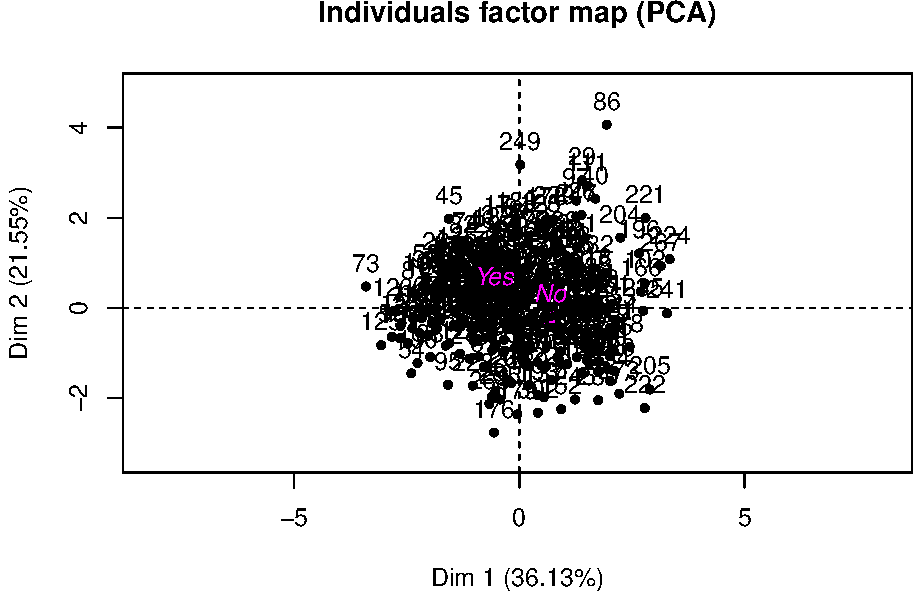
\includegraphics{project_report_files/figure-latex/unnamed-chunk-9-1.pdf}

\begin{Shaded}
\begin{Highlighting}[]
\KeywordTok{plot.PCA}\NormalTok{(pca_facto_heart, }\DataTypeTok{quali.sup =} \DecValTok{6}\NormalTok{, }\DataTypeTok{scale.unit =} \OtherTok{TRUE}\NormalTok{,}\DataTypeTok{choix =} \StringTok{'ind'}\NormalTok{,}\DataTypeTok{label=}\StringTok{"quali"}\NormalTok{)}
\end{Highlighting}
\end{Shaded}

\begin{verbatim}
## Warning in plot.window(...): "quali.sup" is not a graphical parameter
\end{verbatim}

\begin{verbatim}
## Warning in plot.window(...): "scale.unit" is not a graphical parameter
\end{verbatim}

\begin{verbatim}
## Warning in plot.xy(xy, type, ...): "quali.sup" is not a graphical parameter
\end{verbatim}

\begin{verbatim}
## Warning in plot.xy(xy, type, ...): "scale.unit" is not a graphical
## parameter
\end{verbatim}

\begin{verbatim}
## Warning in axis(side = side, at = at, labels = labels, ...): "quali.sup" is
## not a graphical parameter
\end{verbatim}

\begin{verbatim}
## Warning in axis(side = side, at = at, labels = labels, ...): "scale.unit"
## is not a graphical parameter
\end{verbatim}

\begin{verbatim}
## Warning in axis(side = side, at = at, labels = labels, ...): "quali.sup" is
## not a graphical parameter
\end{verbatim}

\begin{verbatim}
## Warning in axis(side = side, at = at, labels = labels, ...): "scale.unit"
## is not a graphical parameter
\end{verbatim}

\begin{verbatim}
## Warning in box(...): "quali.sup" is not a graphical parameter
\end{verbatim}

\begin{verbatim}
## Warning in box(...): "scale.unit" is not a graphical parameter
\end{verbatim}

\begin{verbatim}
## Warning in title(...): "quali.sup" is not a graphical parameter
\end{verbatim}

\begin{verbatim}
## Warning in title(...): "scale.unit" is not a graphical parameter
\end{verbatim}

\begin{verbatim}
## Warning in int_abline(a = a, b = b, h = h, v = v, untf = untf, ...):
## "quali.sup" is not a graphical parameter
\end{verbatim}

\begin{verbatim}
## Warning in int_abline(a = a, b = b, h = h, v = v, untf = untf, ...):
## "scale.unit" is not a graphical parameter
\end{verbatim}

\begin{verbatim}
## Warning in int_abline(a = a, b = b, h = h, v = v, untf = untf, ...):
## "quali.sup" is not a graphical parameter
\end{verbatim}

\begin{verbatim}
## Warning in int_abline(a = a, b = b, h = h, v = v, untf = untf, ...):
## "scale.unit" is not a graphical parameter
\end{verbatim}

\begin{verbatim}
## Warning in plot.xy(xy.coords(x, y), type = type, ...): "quali.sup" is not a
## graphical parameter
\end{verbatim}

\begin{verbatim}
## Warning in plot.xy(xy.coords(x, y), type = type, ...): "scale.unit" is not
## a graphical parameter
\end{verbatim}

\begin{verbatim}
## Warning in text.default(xy, labels, cex = cex, ...): "quali.sup" is not a
## graphical parameter
\end{verbatim}

\begin{verbatim}
## Warning in text.default(xy, labels, cex = cex, ...): "scale.unit" is not a
## graphical parameter
\end{verbatim}

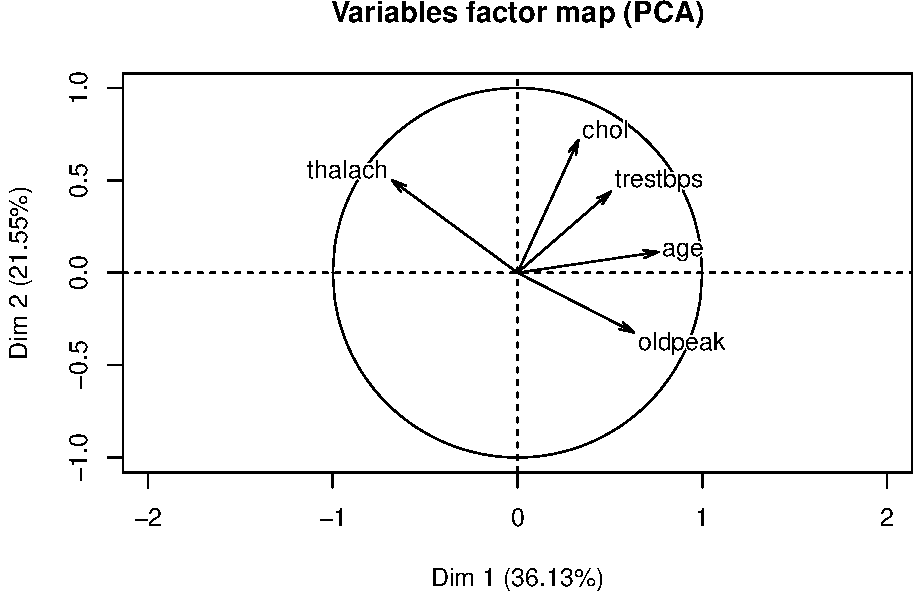
\includegraphics{project_report_files/figure-latex/unnamed-chunk-9-2.pdf}

\begin{Shaded}
\begin{Highlighting}[]
\CommentTok{#Represented in Rn}
\CommentTok{#Projection of variables, show correlation between principal components}
\KeywordTok{fviz_pca_var}\NormalTok{(pca_facto_heart, }\DataTypeTok{geom =} \KeywordTok{c}\NormalTok{(}\StringTok{"arrow"}\NormalTok{, }\StringTok{"text"}\NormalTok{), }\DataTypeTok{col.var =} \StringTok{"cos2"}\NormalTok{)}\CommentTok{#By quality of representation cos2}
\end{Highlighting}
\end{Shaded}

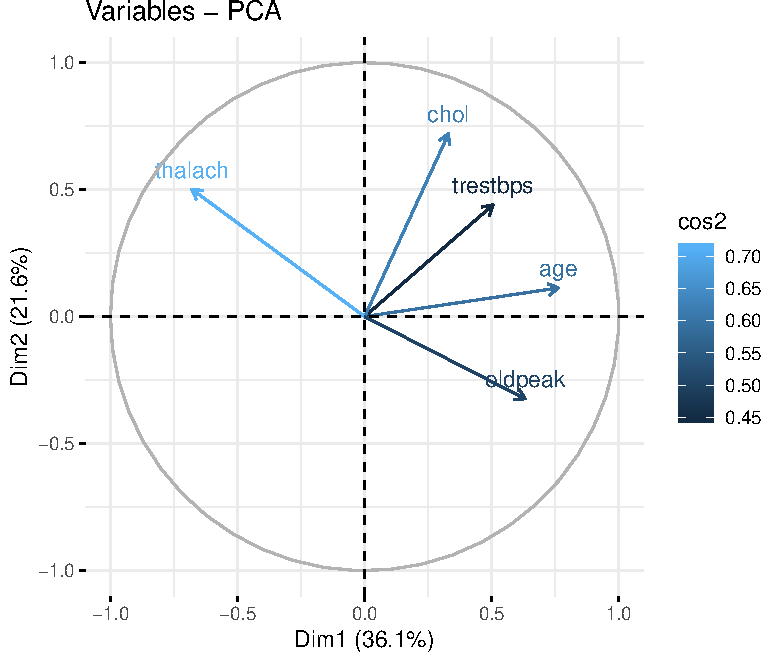
\includegraphics{project_report_files/figure-latex/unnamed-chunk-10-1.pdf}

\begin{Shaded}
\begin{Highlighting}[]
\NormalTok{proj_indiv <-}\StringTok{ }\NormalTok{pca_facto_heart}\OperatorTok{$}\NormalTok{ind}\OperatorTok{$}\NormalTok{coord[,}\DecValTok{1}\OperatorTok{:}\DecValTok{2}\NormalTok{] }\CommentTok{#individual projections on 1st factorial plane}
\CommentTok{#Clustering}
\NormalTok{hc_ward =}\StringTok{ }\KeywordTok{hclust}\NormalTok{(}\KeywordTok{dist}\NormalTok{(proj_indiv),}\DataTypeTok{method =} \StringTok{"ward.D"}\NormalTok{)}
\KeywordTok{plot}\NormalTok{(hc_ward, }\DataTypeTok{main=} \StringTok{"HC using Ward Agglomeration method"}\NormalTok{, }\DataTypeTok{xlab=}\StringTok{""}\NormalTok{,}\DataTypeTok{sub=}\StringTok{""}\NormalTok{,}\DataTypeTok{cex=}\NormalTok{.}\DecValTok{9}\NormalTok{,  }\DataTypeTok{labels=}\OtherTok{FALSE}\NormalTok{)}
\KeywordTok{abline}\NormalTok{(}\DataTypeTok{h=}\DecValTok{60}\NormalTok{)}
\KeywordTok{rect.hclust}\NormalTok{(hc_ward, }\DataTypeTok{k =} \DecValTok{3}\NormalTok{, }\DataTypeTok{border =} \DecValTok{2}\OperatorTok{:}\DecValTok{6}\NormalTok{)}
\end{Highlighting}
\end{Shaded}

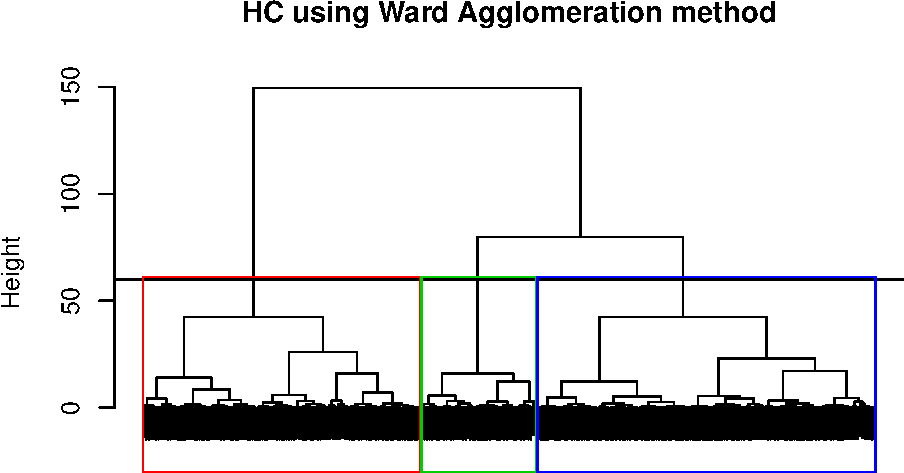
\includegraphics{project_report_files/figure-latex/unnamed-chunk-11-1.pdf}

\begin{Shaded}
\begin{Highlighting}[]
\CommentTok{#Association of individuals to clusters}
\NormalTok{classes <-}\StringTok{ }\KeywordTok{cutree}\NormalTok{(hc_ward, }\DataTypeTok{h=}\DecValTok{50}\NormalTok{) }\CommentTok{#Depending on the height, number of clusters is chosen}
\KeywordTok{plotcluster}\NormalTok{(proj_indiv, classes,}\DataTypeTok{main=}\StringTok{"Projections of individuals in Hierarchical Clustering of 3 classes"}\NormalTok{)}
\end{Highlighting}
\end{Shaded}

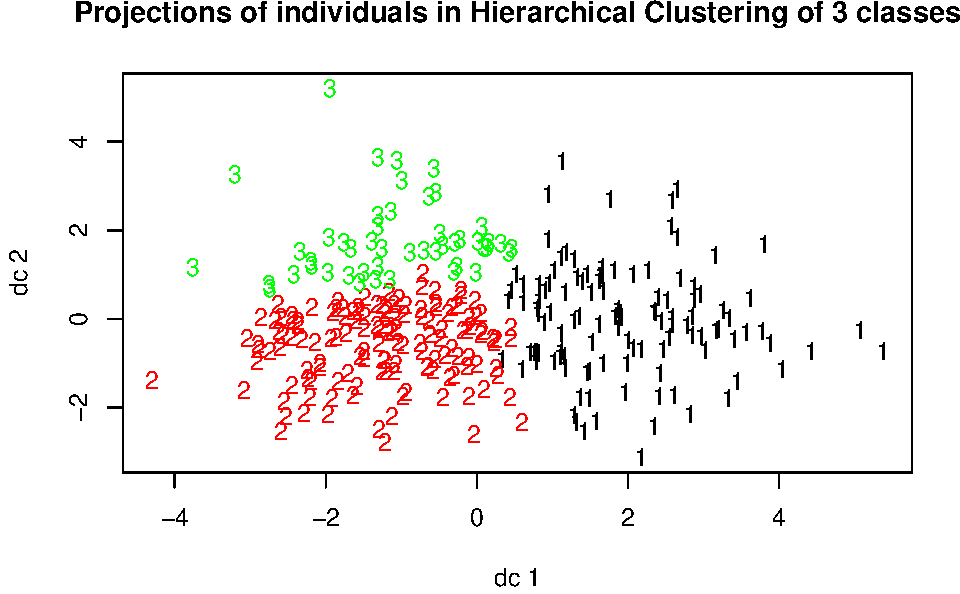
\includegraphics{project_report_files/figure-latex/unnamed-chunk-11-2.pdf}

\begin{Shaded}
\begin{Highlighting}[]
\NormalTok{get_centroids <-}\StringTok{ }\ControlFlowTok{function}\NormalTok{(classes, n_classes)\{}
\NormalTok{  centroids <-}\StringTok{ }\OtherTok{NULL}
  \ControlFlowTok{for}\NormalTok{(k }\ControlFlowTok{in} \DecValTok{1}\OperatorTok{:}\NormalTok{n_classes)\{}
\NormalTok{    centroids <-}\StringTok{ }\KeywordTok{rbind}\NormalTok{(centroids, }\KeywordTok{colMeans}\NormalTok{(proj_indiv[classes }\OperatorTok{==}\StringTok{ }\NormalTok{k, , }\DataTypeTok{drop =} \OtherTok{FALSE}\NormalTok{]))}
\NormalTok{  \}}
  \KeywordTok{return}\NormalTok{(centroids)}
\NormalTok{\}}
\NormalTok{centroids <-}\StringTok{ }\KeywordTok{get_centroids}\NormalTok{(classes, }\DecValTok{3}\NormalTok{)}
\end{Highlighting}
\end{Shaded}

\begin{Shaded}
\begin{Highlighting}[]
\CommentTok{#k_mean needs centroid of clusters}
\NormalTok{k_mean <-}\StringTok{ }\KeywordTok{kmeans}\NormalTok{(proj_indiv, centroids)}
\KeywordTok{plotcluster}\NormalTok{(proj_indiv, k_mean}\OperatorTok{$}\NormalTok{cluster,}\DataTypeTok{main=}\StringTok{"Projections of individuals in K-means Clustering of 3 classes"}\NormalTok{)}
\end{Highlighting}
\end{Shaded}

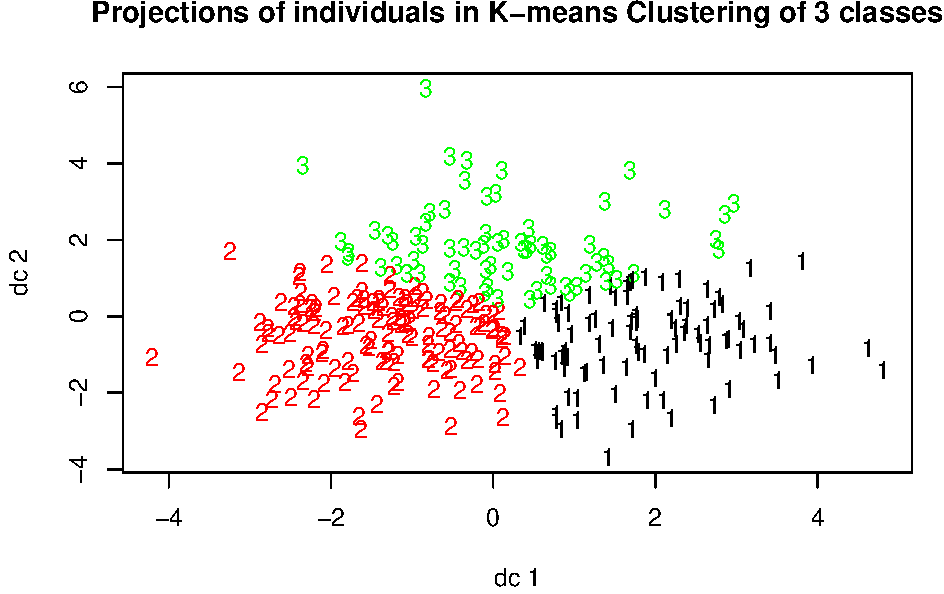
\includegraphics{project_report_files/figure-latex/unnamed-chunk-13-1.pdf}

\begin{Shaded}
\begin{Highlighting}[]
\NormalTok{cal_idx_before <-}\StringTok{ }\KeywordTok{calinhara}\NormalTok{(proj_indiv,classes,}\DataTypeTok{cn=}\KeywordTok{max}\NormalTok{(classes))}
\NormalTok{cal_idx_after <-}\StringTok{ }\KeywordTok{calinhara}\NormalTok{(proj_indiv,k_mean}\OperatorTok{$}\NormalTok{cluster,}\DataTypeTok{cn=}\KeywordTok{max}\NormalTok{(k_mean}\OperatorTok{$}\NormalTok{cluster))}

\KeywordTok{print}\NormalTok{(cal_idx_before)}
\end{Highlighting}
\end{Shaded}

\begin{verbatim}
## [1] 198.1154
\end{verbatim}

\begin{Shaded}
\begin{Highlighting}[]
\KeywordTok{print}\NormalTok{(cal_idx_after)}
\end{Highlighting}
\end{Shaded}

\begin{verbatim}
## [1] 226.1952
\end{verbatim}

\begin{Shaded}
\begin{Highlighting}[]
\CommentTok{#Improvement}
\end{Highlighting}
\end{Shaded}

\begin{Shaded}
\begin{Highlighting}[]
\NormalTok{Calinski_Harabassza <-}\StringTok{ }\ControlFlowTok{function}\NormalTok{ (projections, hc, kind, n_classes)\{}
\NormalTok{  classes <-}\StringTok{ }\KeywordTok{cutree}\NormalTok{(hc, }\DataTypeTok{k=}\NormalTok{n_classes)}
\NormalTok{  centroids <-}\StringTok{ }\KeywordTok{get_centroids}\NormalTok{(classes, n_classes)}
  \ControlFlowTok{if}\NormalTok{(kind}\OperatorTok{==}\StringTok{'hc'}\NormalTok{)\{}
\NormalTok{    index <-}\StringTok{ }\KeywordTok{calinhara}\NormalTok{(proj_indiv,classes,}\DataTypeTok{cn=}\KeywordTok{max}\NormalTok{(classes))}
\NormalTok{  \}}
  \ControlFlowTok{if}\NormalTok{(kind}\OperatorTok{==}\StringTok{'kmeans'}\NormalTok{)\{}
\NormalTok{    kmeans_classes <-}\StringTok{ }\KeywordTok{kmeans}\NormalTok{(proj_indiv, }\DataTypeTok{centers =}\NormalTok{ centroids)}\OperatorTok{$}\NormalTok{cluster}
\NormalTok{    index <-}\KeywordTok{calinhara}\NormalTok{(proj_indiv,kmeans_classes,}\DataTypeTok{cn=}\KeywordTok{max}\NormalTok{(kmeans_classes)) }
\NormalTok{  \}}
  \KeywordTok{return}\NormalTok{(index)}
\NormalTok{\}}
\NormalTok{get_indexes <-}\StringTok{ }\ControlFlowTok{function}\NormalTok{(until, kind)\{}
\NormalTok{  indexes <-}\StringTok{ }\KeywordTok{c}\NormalTok{()}
  \ControlFlowTok{for}\NormalTok{ (n_classes }\ControlFlowTok{in} \DecValTok{2}\OperatorTok{:}\NormalTok{until)\{}
\NormalTok{    indexes <-}\StringTok{ }\KeywordTok{c}\NormalTok{(indexes, }\KeywordTok{Calinski_Harabassza}\NormalTok{(proj_indiv, hc_ward, kind, n_classes))}
\NormalTok{  \}  }
  \KeywordTok{return}\NormalTok{(indexes)}
\NormalTok{\}}
\end{Highlighting}
\end{Shaded}

\begin{Shaded}
\begin{Highlighting}[]
\NormalTok{indexes_before <-}\StringTok{ }\KeywordTok{get_indexes}\NormalTok{(}\DecValTok{10}\NormalTok{, }\StringTok{'hc'}\NormalTok{)}
\KeywordTok{plot}\NormalTok{(indexes_before, }\DataTypeTok{type =} \StringTok{"o"}\NormalTok{, }\DataTypeTok{xlab =} \StringTok{'Number of classes'}\NormalTok{, }\DataTypeTok{ylab =} \StringTok{'Calinski index value'}
\NormalTok{, }\DataTypeTok{main =} \StringTok{'Index before consolidation'}\NormalTok{, }\DataTypeTok{col =} \StringTok{'blue'}\NormalTok{, xaxt}
\NormalTok{=}\StringTok{ "n"}\NormalTok{)}
\KeywordTok{axis}\NormalTok{(}\DecValTok{1}\NormalTok{, }\DataTypeTok{at=}\DecValTok{1}\OperatorTok{:}\DecValTok{9}\NormalTok{, }\DataTypeTok{labels =} \KeywordTok{c}\NormalTok{(}\DecValTok{2}\NormalTok{, }\DecValTok{3}\NormalTok{, }\DecValTok{4}\NormalTok{, }\DecValTok{5}\NormalTok{, }\DecValTok{6}\NormalTok{, }\DecValTok{7}\NormalTok{,}\DecValTok{8}\NormalTok{,}\DecValTok{9}\NormalTok{,}\DecValTok{10}\NormalTok{))  }
\end{Highlighting}
\end{Shaded}

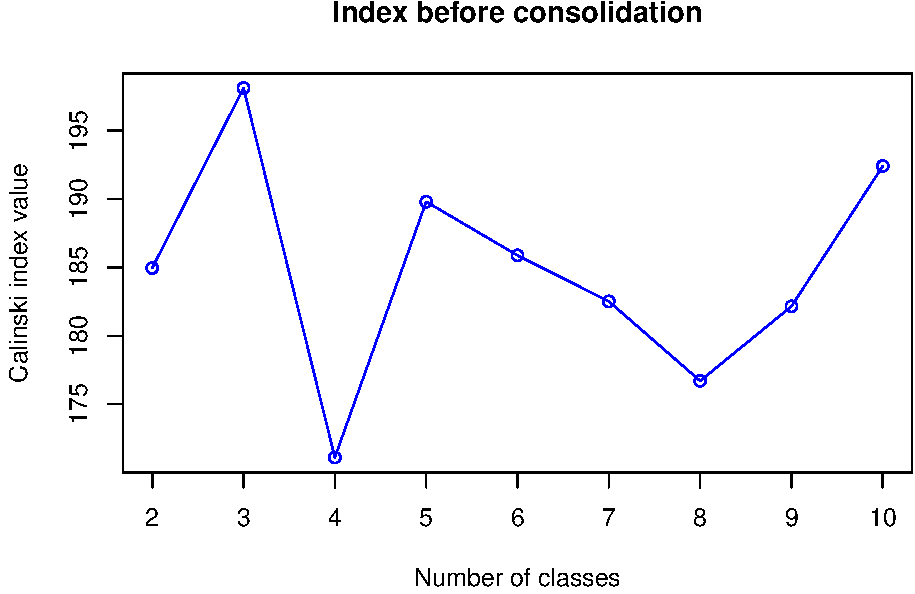
\includegraphics{project_report_files/figure-latex/unnamed-chunk-16-1.pdf}

\begin{Shaded}
\begin{Highlighting}[]
\NormalTok{indexes_after <-}\StringTok{ }\KeywordTok{get_indexes}\NormalTok{(}\DecValTok{10}\NormalTok{, }\StringTok{'kmeans'}\NormalTok{)}
\KeywordTok{plot}\NormalTok{(indexes_after, }\DataTypeTok{type =} \StringTok{"o"}\NormalTok{, }\DataTypeTok{xlab =} \StringTok{'Number of classes'}\NormalTok{, }\DataTypeTok{ylab =} \StringTok{'Calinski index value'}
\NormalTok{, }\DataTypeTok{main =} \StringTok{'Index after consolidation'}\NormalTok{, }\DataTypeTok{col =} \StringTok{'blue'}\NormalTok{, xaxt}
\NormalTok{=}\StringTok{ "n"}\NormalTok{)}
\KeywordTok{axis}\NormalTok{(}\DecValTok{1}\NormalTok{, }\DataTypeTok{at=}\DecValTok{1}\OperatorTok{:}\DecValTok{9}\NormalTok{, }\DataTypeTok{labels =} \KeywordTok{c}\NormalTok{(}\DecValTok{2}\NormalTok{, }\DecValTok{3}\NormalTok{, }\DecValTok{4}\NormalTok{, }\DecValTok{5}\NormalTok{, }\DecValTok{6}\NormalTok{, }\DecValTok{7}\NormalTok{,}\DecValTok{8}\NormalTok{,}\DecValTok{9}\NormalTok{,}\DecValTok{10}\NormalTok{))  }
\end{Highlighting}
\end{Shaded}

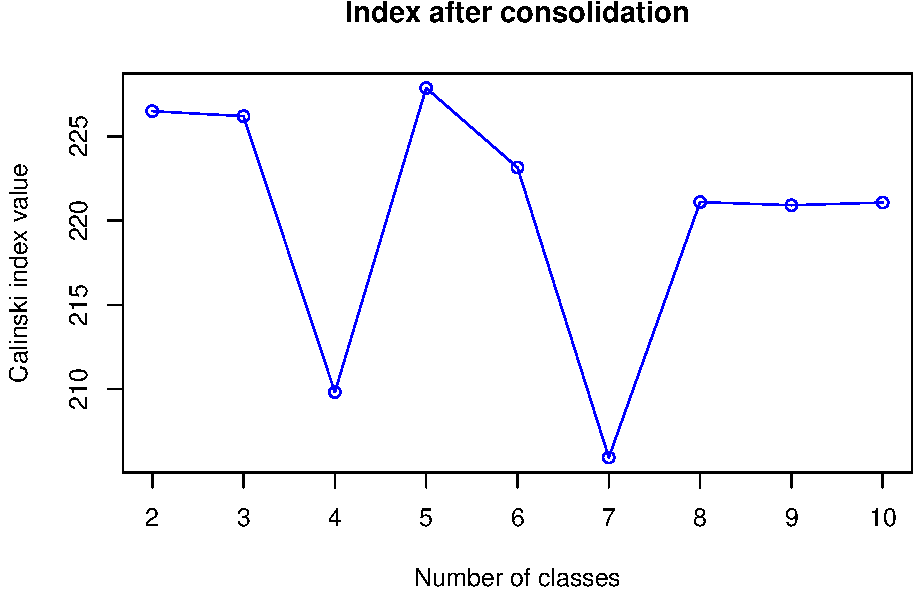
\includegraphics{project_report_files/figure-latex/unnamed-chunk-17-1.pdf}

\begin{Shaded}
\begin{Highlighting}[]
\NormalTok{first_factorial <-}\StringTok{ }\NormalTok{proj_indiv}
\NormalTok{df <-}\StringTok{ }\KeywordTok{data.frame}\NormalTok{(first_factorial, }\DataTypeTok{Class =} \KeywordTok{as.factor}\NormalTok{(k_mean}\OperatorTok{$}\NormalTok{cluster))}
\KeywordTok{catdes}\NormalTok{(df, }\DataTypeTok{num.var =} \KeywordTok{length}\NormalTok{(df), }\DataTypeTok{proba =} \FloatTok{0.05}\NormalTok{, }\DataTypeTok{row.w =} \OtherTok{NULL}\NormalTok{)}
\end{Highlighting}
\end{Shaded}

\begin{verbatim}
## 
## Link between the cluster variable and the quantitative variables
## ================================================================
##            Eta2      P-value
## Dim.1 0.6316289 8.766734e-66
## Dim.2 0.5503737 8.467640e-53
## 
## Description of each cluster by quantitative variables
## =====================================================
## $`1`
##           v.test Mean in category  Overall mean sd in category Overall sd
## Dim.1   9.014585        1.0477037  2.852366e-15      0.8712730   1.344089
## Dim.2 -10.516103       -0.9439256 -3.090499e-16      0.6923393   1.038050
##            p.value
## Dim.1 1.976176e-19
## Dim.2 7.282354e-26
## 
## $`2`
##          v.test Mean in category Overall mean sd in category Overall sd
## Dim.1 -13.79634        -1.151379 2.852366e-15      0.7373691   1.344089
##            p.value
## Dim.1 2.681253e-43
## 
## $`3`
##          v.test Mean in category  Overall mean sd in category Overall sd
## Dim.2 10.780147        1.1748120 -3.090499e-16      0.7675912   1.038050
## Dim.1  6.454662        0.9108084  2.852366e-15      0.8858076   1.344089
##            p.value
## Dim.2 4.272002e-27
## Dim.1 1.084604e-10
\end{verbatim}

\begin{Shaded}
\begin{Highlighting}[]
\NormalTok{factor_heart}\OperatorTok{$}\NormalTok{disease[factor_heart}\OperatorTok{$}\NormalTok{target}\OperatorTok{==}\DecValTok{0}\NormalTok{] <-}\StringTok{ "Yes"}
\NormalTok{factor_heart}\OperatorTok{$}\NormalTok{disease[factor_heart}\OperatorTok{$}\NormalTok{target}\OperatorTok{==}\DecValTok{1}\NormalTok{] <-}\StringTok{ "No"}
\NormalTok{factor_heart}\OperatorTok{$}\NormalTok{target <-}\StringTok{ }\OtherTok{NULL}

\NormalTok{factor_heart2 <-}\StringTok{ }\NormalTok{factor_heart}
\NormalTok{factor_heart2}\OperatorTok{$}\NormalTok{age<-}\KeywordTok{cut}\NormalTok{(factor_heart2}\OperatorTok{$}\NormalTok{age, }\KeywordTok{seq}\NormalTok{(}\DecValTok{0}\NormalTok{,}\DecValTok{80}\NormalTok{,}\DecValTok{10}\NormalTok{), }\DataTypeTok{right=}\OtherTok{FALSE}\NormalTok{)}
\NormalTok{factor_heart2}\OperatorTok{$}\NormalTok{age <-}\StringTok{ }\KeywordTok{paste}\NormalTok{(}\StringTok{"Age"}\NormalTok{, factor_heart2}\OperatorTok{$}\NormalTok{age, }\DataTypeTok{sep=}\StringTok{"_"}\NormalTok{)}
\KeywordTok{min}\NormalTok{(factor_heart2}\OperatorTok{$}\NormalTok{oldpeak)}
\end{Highlighting}
\end{Shaded}

\begin{verbatim}
## [1] 0
\end{verbatim}

\begin{Shaded}
\begin{Highlighting}[]
\NormalTok{factor_heart2}\OperatorTok{$}\NormalTok{oldpeak<-}\KeywordTok{cut}\NormalTok{(factor_heart2}\OperatorTok{$}\NormalTok{oldpeak, }\KeywordTok{seq}\NormalTok{(}\DecValTok{0}\NormalTok{,}\DecValTok{7}\NormalTok{,}\DecValTok{1}\NormalTok{), }\DataTypeTok{right=}\OtherTok{FALSE}\NormalTok{)}
\NormalTok{factor_heart2}\OperatorTok{$}\NormalTok{oldpeak <-}\StringTok{ }\KeywordTok{paste}\NormalTok{(}\StringTok{"Oldp"}\NormalTok{, factor_heart2}\OperatorTok{$}\NormalTok{oldpeak, }\DataTypeTok{sep=}\StringTok{"_"}\NormalTok{)}
\NormalTok{factor_heart2}\OperatorTok{$}\NormalTok{thalach<-}\KeywordTok{cut}\NormalTok{(factor_heart2}\OperatorTok{$}\NormalTok{thalach, }\KeywordTok{seq}\NormalTok{(}\DecValTok{70}\NormalTok{,}\DecValTok{220}\NormalTok{,}\DecValTok{20}\NormalTok{), }\DataTypeTok{right=}\OtherTok{FALSE}\NormalTok{)}
\NormalTok{factor_heart2}\OperatorTok{$}\NormalTok{thalach <-}\StringTok{ }\KeywordTok{paste}\NormalTok{(}\StringTok{"thalach"}\NormalTok{, factor_heart2}\OperatorTok{$}\NormalTok{thalach, }\DataTypeTok{sep=}\StringTok{"_"}\NormalTok{)}
\NormalTok{factor_heart2}\OperatorTok{$}\NormalTok{trestbps<-}\KeywordTok{cut}\NormalTok{(factor_heart2}\OperatorTok{$}\NormalTok{trestbps, }\KeywordTok{seq}\NormalTok{(}\DecValTok{80}\NormalTok{,}\DecValTok{220}\NormalTok{,}\DecValTok{20}\NormalTok{), }\DataTypeTok{right=}\OtherTok{FALSE}\NormalTok{)}
\NormalTok{factor_heart2}\OperatorTok{$}\NormalTok{trestbps <-}\StringTok{ }\KeywordTok{paste}\NormalTok{(}\StringTok{"thres"}\NormalTok{, factor_heart2}\OperatorTok{$}\NormalTok{trestbps, }\DataTypeTok{sep=}\StringTok{"_"}\NormalTok{)}
\NormalTok{factor_heart2}\OperatorTok{$}\NormalTok{chol<-}\KeywordTok{cut}\NormalTok{(factor_heart2}\OperatorTok{$}\NormalTok{chol, }\KeywordTok{seq}\NormalTok{(}\DecValTok{100}\NormalTok{,}\DecValTok{600}\NormalTok{,}\DecValTok{100}\NormalTok{), }\DataTypeTok{right=}\OtherTok{FALSE}\NormalTok{)}
\NormalTok{factor_heart2}\OperatorTok{$}\NormalTok{chol <-}\StringTok{ }\KeywordTok{paste}\NormalTok{(}\StringTok{"Col"}\NormalTok{, factor_heart2}\OperatorTok{$}\NormalTok{chol, }\DataTypeTok{sep=}\StringTok{"_"}\NormalTok{)}
\CommentTok{#factor_heart2$age <- NULL}
\KeywordTok{kable}\NormalTok{(}\KeywordTok{head}\NormalTok{(factor_heart2))}
\end{Highlighting}
\end{Shaded}

\begin{longtable}[]{@{}llllllllllllll@{}}
\toprule
age & sex & cp & trestbps & chol & fbs & restecg & thalach & exang &
oldpeak & slope & ca & thal & disease\tabularnewline
\midrule
\endhead
Age\_{[}60,70) & 1 & 3 & thres\_{[}140,160) & Col\_{[}200,300) & 1 & 0 &
thalach\_{[}150,170) & 0 & Oldp\_{[}2,3) & 0 & 0 & 1 & No\tabularnewline
Age\_{[}30,40) & 1 & 2 & thres\_{[}120,140) & Col\_{[}200,300) & 0 & 1 &
thalach\_{[}170,190) & 0 & Oldp\_{[}3,4) & 0 & 0 & 2 & No\tabularnewline
Age\_{[}40,50) & 0 & 1 & thres\_{[}120,140) & Col\_{[}200,300) & 0 & 0 &
thalach\_{[}170,190) & 0 & Oldp\_{[}1,2) & 2 & 0 & 2 & No\tabularnewline
Age\_{[}50,60) & 1 & 1 & thres\_{[}120,140) & Col\_{[}200,300) & 0 & 1 &
thalach\_{[}170,190) & 0 & Oldp\_{[}0,1) & 2 & 0 & 2 & No\tabularnewline
Age\_{[}50,60) & 0 & 0 & thres\_{[}120,140) & Col\_{[}300,400) & 0 & 1 &
thalach\_{[}150,170) & 1 & Oldp\_{[}0,1) & 2 & 0 & 2 & No\tabularnewline
Age\_{[}50,60) & 1 & 0 & thres\_{[}140,160) & Col\_{[}100,200) & 0 & 1 &
thalach\_{[}130,150) & 0 & Oldp\_{[}0,1) & 1 & 0 & 1 & No\tabularnewline
\bottomrule
\end{longtable}

\begin{Shaded}
\begin{Highlighting}[]
\NormalTok{mcaHeart <-}\StringTok{ }\KeywordTok{MCA}\NormalTok{(factor_heart2,}\DataTypeTok{ncp=}\DecValTok{7}\NormalTok{,}
               \CommentTok{#quanti.sup=c(10),}
               \DataTypeTok{quali.sup=}\KeywordTok{c}\NormalTok{(}\DecValTok{14}\NormalTok{),}
               \DataTypeTok{excl=}\OtherTok{NULL}\NormalTok{,}
               \DataTypeTok{graph =} \OtherTok{FALSE}\NormalTok{,}
               \DataTypeTok{level.ventil =} \FloatTok{0.00}\NormalTok{,}
               \DataTypeTok{axes =} \KeywordTok{c}\NormalTok{(}\DecValTok{1}\NormalTok{,}\DecValTok{2}\NormalTok{),}
               \DataTypeTok{row.w =} \OtherTok{NULL}\NormalTok{,}
               \DataTypeTok{method=}\StringTok{"Indicator"}\NormalTok{,}
               \DataTypeTok{na.method=}\StringTok{"NA"}\NormalTok{,}
               \DataTypeTok{tab.disj=}\OtherTok{NULL}\NormalTok{)}

\CommentTok{# mcaHeart <- MCA(factor_heart,ncp=7,}
\CommentTok{#                quanti.sup=c(1,4,5,8,10),}
\CommentTok{#                quali.sup=c(14),}
\CommentTok{#                excl=NULL,}
\CommentTok{#                graph = FALSE,}
\CommentTok{#                level.ventil = 0.00,}
\CommentTok{#                axes = c(1,2),}
\CommentTok{#                row.w = NULL,}
\CommentTok{#                method="Indicator",}
\CommentTok{#                na.method="NA",}
\CommentTok{#                tab.disj=NULL)}
\KeywordTok{summary}\NormalTok{(mcaHeart)}
\end{Highlighting}
\end{Shaded}

\begin{verbatim}
## 
## Call:
## MCA(X = factor_heart2, ncp = 7, quali.sup = c(14), excl = NULL,  
##      graph = FALSE, level.ventil = 0, axes = c(1, 2), row.w = NULL,  
##      method = "Indicator", na.method = "NA", tab.disj = NULL) 
## 
## 
## Eigenvalues
##                        Dim.1   Dim.2   Dim.3   Dim.4   Dim.5   Dim.6
## Variance               0.264   0.142   0.134   0.129   0.126   0.119
## % of var.              7.805   4.192   3.961   3.803   3.736   3.513
## Cumulative % of var.   7.805  11.997  15.958  19.761  23.496  27.009
##                        Dim.7   Dim.8   Dim.9  Dim.10  Dim.11  Dim.12
## Variance               0.110   0.108   0.106   0.101   0.097   0.096
## % of var.              3.263   3.188   3.131   2.981   2.869   2.844
## Cumulative % of var.  30.273  33.460  36.592  39.573  42.442  45.286
##                       Dim.13  Dim.14  Dim.15  Dim.16  Dim.17  Dim.18
## Variance               0.093   0.090   0.088   0.085   0.081   0.079
## % of var.              2.759   2.661   2.587   2.521   2.390   2.332
## Cumulative % of var.  48.045  50.706  53.293  55.814  58.204  60.536
##                       Dim.19  Dim.20  Dim.21  Dim.22  Dim.23  Dim.24
## Variance               0.079   0.077   0.075   0.072   0.070   0.068
## % of var.              2.322   2.283   2.213   2.140   2.079   1.997
## Cumulative % of var.  62.858  65.141  67.355  69.495  71.574  73.571
##                       Dim.25  Dim.26  Dim.27  Dim.28  Dim.29  Dim.30
## Variance               0.066   0.064   0.063   0.060   0.057   0.055
## % of var.              1.950   1.891   1.850   1.782   1.693   1.635
## Cumulative % of var.  75.521  77.412  79.262  81.043  82.736  84.371
##                       Dim.31  Dim.32  Dim.33  Dim.34  Dim.35  Dim.36
## Variance               0.054   0.052   0.050   0.046   0.044   0.040
## % of var.              1.596   1.543   1.491   1.364   1.291   1.192
## Cumulative % of var.  85.968  87.511  89.002  90.366  91.657  92.849
##                       Dim.37  Dim.38  Dim.39  Dim.40  Dim.41  Dim.42
## Variance               0.039   0.037   0.034   0.031   0.029   0.026
## % of var.              1.138   1.085   1.008   0.916   0.852   0.771
## Cumulative % of var.  93.987  95.072  96.080  96.996  97.848  98.619
##                       Dim.43  Dim.44
## Variance               0.024   0.023
## % of var.              0.712   0.669
## Cumulative % of var.  99.331 100.000
## 
## Individuals (the 10 first)
##                Dim.1    ctr   cos2    Dim.2    ctr   cos2    Dim.3    ctr
## 1           |  0.527  0.347  0.055 |  0.515  0.618  0.052 |  0.515  0.652
## 2           | -0.428  0.229  0.039 |  0.110  0.028  0.003 |  0.790  1.537
## 3           | -0.681  0.579  0.257 |  0.057  0.008  0.002 | -0.091  0.020
## 4           | -0.718  0.645  0.376 | -0.104  0.025  0.008 |  0.229  0.129
## 5           | -0.262  0.086  0.043 |  0.111  0.029  0.008 | -0.379  0.354
## 6           |  0.229  0.065  0.020 | -0.107  0.027  0.004 |  0.451  0.500
## 7           | -0.206  0.053  0.026 |  0.191  0.085  0.022 | -0.453  0.505
## 8           | -0.656  0.538  0.274 | -0.209  0.101  0.028 |  0.359  0.318
## 9           | -0.194  0.047  0.014 |  0.300  0.210  0.032 |  0.204  0.102
## 10          | -0.484  0.293  0.126 | -0.003  0.000  0.000 |  0.079  0.015
##               cos2  
## 1            0.052 |
## 2            0.132 |
## 3            0.005 |
## 4            0.038 |
## 5            0.090 |
## 6            0.076 |
## 7            0.124 |
## 8            0.082 |
## 9            0.015 |
## 10           0.003 |
## 
## Categories (the 10 first)
##                Dim.1    ctr   cos2 v.test    Dim.2    ctr   cos2 v.test  
## Age_[20,30) | -1.800  0.311  0.011 -1.800 |  0.241  0.010  0.000  0.241 |
## Age_[30,40) | -1.140  1.873  0.068 -4.521 | -0.337  0.305  0.006 -1.338 |
## Age_[40,50) | -0.641  2.839  0.128 -6.214 | -0.230  0.679  0.016 -2.228 |
## Age_[50,60) |  0.158  0.299  0.017  2.298 | -0.011  0.003  0.000 -0.165 |
## Age_[60,70) |  0.532  2.178  0.102  5.540 |  0.246  0.865  0.022  2.559 |
## Age_[70,80) |  0.271  0.071  0.003  0.870 |  0.310  0.172  0.003  0.996 |
## sex_0       | -0.294  0.798  0.040 -3.481 |  0.588  5.932  0.160  6.955 |
## sex_1       |  0.136  0.370  0.040  3.481 | -0.273  2.751  0.160 -6.955 |
## cp_0        |  0.638  5.586  0.363 10.474 | -0.164  0.687  0.024 -2.692 |
## cp_1        | -0.957  4.396  0.181 -7.390 |  0.035  0.011  0.000  0.271 |
##              Dim.3    ctr   cos2 v.test  
## Age_[20,30)  4.476  3.794  0.066  4.476 |
## Age_[30,40)  1.347  5.156  0.095  5.344 |
## Age_[40,50)  0.305  1.271  0.029  2.962 |
## Age_[50,60)  0.059  0.081  0.002  0.854 |
## Age_[60,70) -0.618  5.780  0.137 -6.429 |
## Age_[70,80) -0.459  0.398  0.007 -1.472 |
## sex_0       -0.721  9.462  0.241 -8.538 |
## sex_1        0.335  4.388  0.241  8.538 |
## cp_0        -0.031  0.026  0.001 -0.505 |
## cp_1         0.247  0.579  0.012  1.911 |
## 
## Categorical variables (eta2)
##               Dim.1 Dim.2 Dim.3  
## age         | 0.260 0.038 0.287 |
## sex         | 0.040 0.160 0.241 |
## cp          | 0.421 0.030 0.047 |
## trestbps    | 0.119 0.313 0.068 |
## chol        | 0.014 0.140 0.228 |
## fbs         | 0.018 0.053 0.002 |
## restecg     | 0.096 0.068 0.002 |
## thalach     | 0.519 0.119 0.314 |
## exang       | 0.336 0.061 0.001 |
## oldpeak     | 0.507 0.476 0.192 |
## 
## Supplementary categories
##                 Dim.1    cos2  v.test     Dim.2    cos2  v.test     Dim.3
## No          |  -0.619   0.458 -11.767 |   0.142   0.024   2.694 |  -0.040
## Yes         |   0.740   0.458  11.767 |  -0.170   0.024  -2.694 |   0.048
##                cos2  v.test  
## No            0.002  -0.766 |
## Yes           0.002   0.766 |
## 
## Supplementary categorical variables (eta2)
##               Dim.1 Dim.2 Dim.3  
## disease     | 0.458 0.024 0.002 |
\end{verbatim}

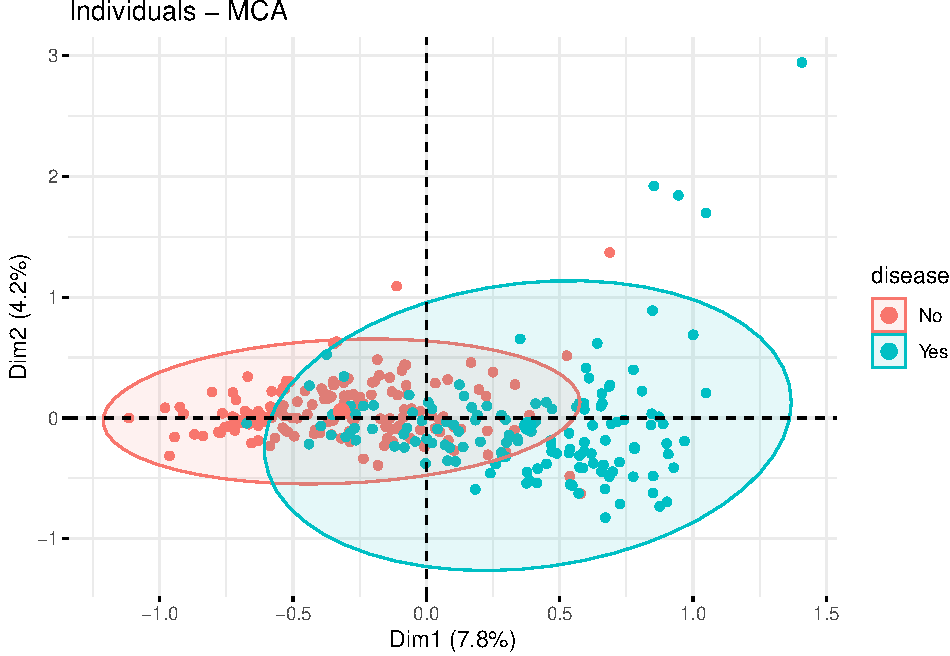
\includegraphics{project_report_files/figure-latex/unnamed-chunk-20-1.pdf}

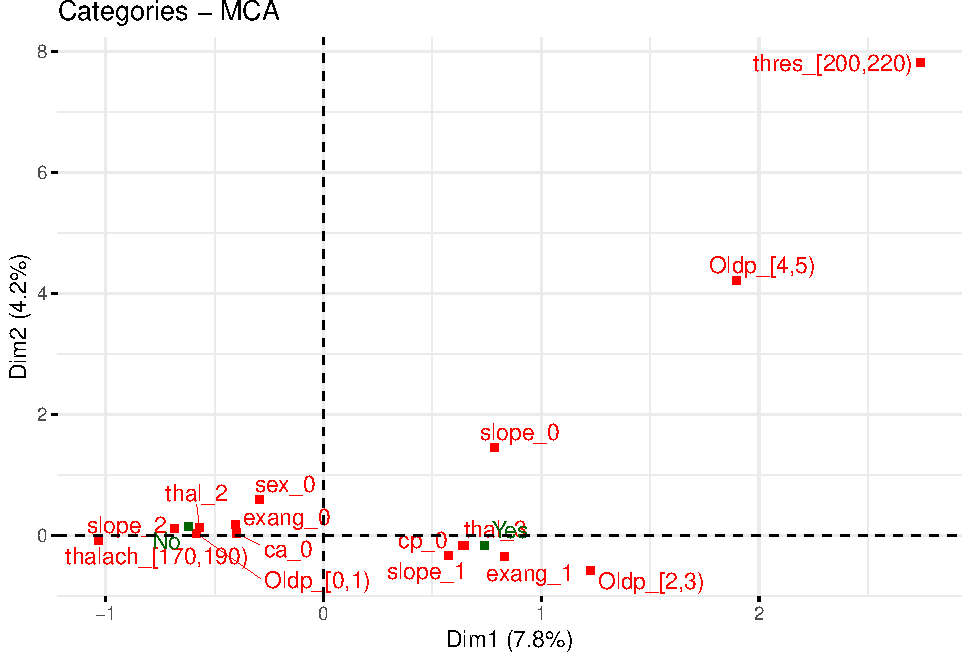
\includegraphics{project_report_files/figure-latex/unnamed-chunk-21-1.pdf}
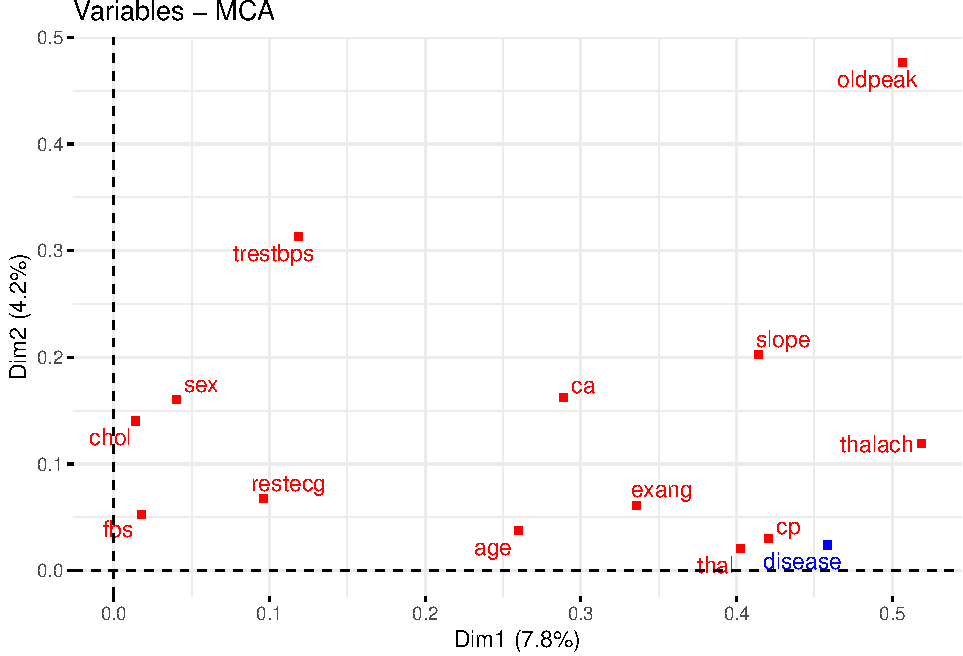
\includegraphics{project_report_files/figure-latex/unnamed-chunk-21-2.pdf}

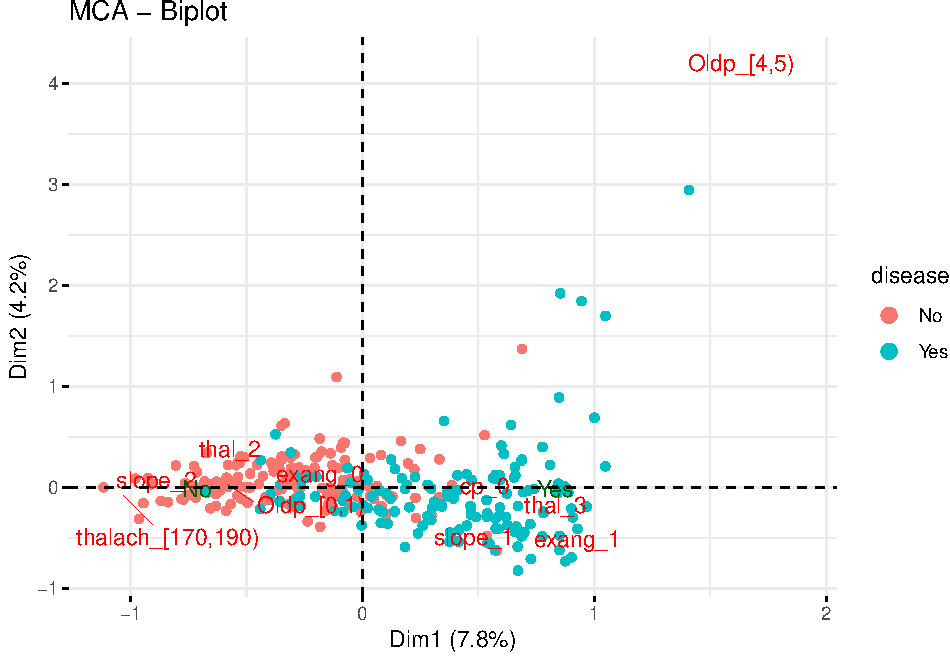
\includegraphics{project_report_files/figure-latex/unnamed-chunk-22-1.pdf}

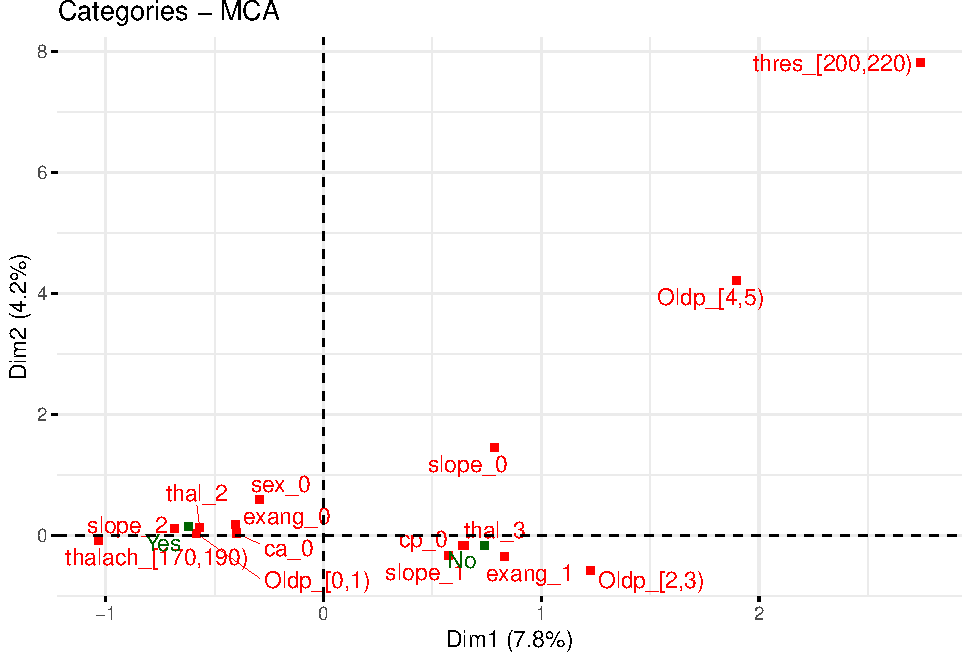
\includegraphics{project_report_files/figure-latex/unnamed-chunk-23-1.pdf}


\end{document}
